%%%%%%%%%%%%%%%%%%%%%%%%%%%%%%%%%%%%%%%%%
% Beamer Presentation
% LaTeX Template
% Version 1.0 (10/11/12)
%
% This template has been downloaded from:
% http://www.LaTeXTemplates.com
%
% License:
% CC BY-NC-SA 3.0 (http://creativecommons.org/licenses/by-nc-sa/3.0/)
%
%%%%%%%%%%%%%%%%%%%%%%%%%%%%%%%%%%%%%%%%%

%----------------------------------------------------------------------------------------
%	PACKAGES AND THEMES
%----------------------------------------------------------------------------------------

\documentclass{beamer}

\mode<presentation> {

\usetheme{Madrid}

%\usecolortheme{beaver}
%\usecolortheme{crane}
%\usecolortheme{dolphin}
%\usecolortheme{rose}
%\usecolortheme{seagull}
\usecolortheme{seahorse}
%\usecolortheme{wolverine}
}

\usepackage[english]{babel}
\usepackage[utf8]{inputenc}
\usepackage{graphicx} % Allows including images
\usepackage{grffile}
\usepackage{booktabs} % Allows the use of \toprule, \midrule and \bottomrule in tables

%----------------------------------------------------------------------------------------
%	TITLE PAGE
%----------------------------------------------------------------------------------------



%----------------------------------------------------------------------------------------%

\title[ROS]{Robotics and ROS} % The short title appears at the bottom of every slide, the full title is only on the title page

\author{Khan Saad Bin Hasan} % Your name
\institute[] % Your institution as it will appear on the bottom of every slide, may be shorthand to save space
{
khansaadbinhasan.github.io \\ % Your institution for the title page
\medskip
\textit{khansaadbinhasan@gmail.com} % Your email address
}
\date{\today} % Date, can be changed to a custom date

\begin{document}
	\begin{frame}
	\titlepage % Print the title page as the first slide
	\end{frame}

	%----------------------------------------------------------------------------------------%


	%----------------------------------------------------------------------------------------%

	\begin{frame}
	\frametitle{Contents} % Table of contents slide, comment this block out to remove it
	\tableofcontents % Throughout your presentation, if you choose to use \section{} and \subsection{} commands, these will automatically be printed on this slide as an overview of your presentation
	\end{frame}

	%----------------------------------------------------------------------------------------%


	%----------------------------------------------------------------------------------------%

	\section{Robotics and ROS}
	\begin{frame}
		\frametitle{General Outline of a Robotic System}
		\subsection{General Outline of a Robotic System}
		\begin{figure}
			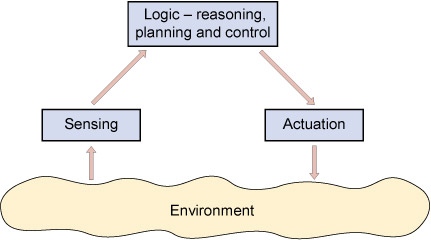
\includegraphics[width=0.8\linewidth]{images/sensing-logic-actuation.jpg}
		\end{figure}
	\end{frame}

	%----------------------------------------------------------------------------------------%


	%----------------------------------------------------------------------------------------%

	\begin{frame}
		\frametitle{Sensors and Actuators}
		\subsection{Sensors and Actuators}

		\begin{itemize}
			\item Sensors can never be perfect.\medskip
			\item Built up of a number of modules, Hence multiple points of failures e.g, LIDARs have a rotating top, a laser sender, a receiver and a PCB.\medskip
			\item Coordination between all the modules may never be perfect.\medskip
			\item The better a sensor is, the costlier it gets. e.g, IMUs% Cheap IMUs and High grade IMUs
			, Cameras etc. %Cheap $10 cameras and high priced Stereo Cameras.
		\end{itemize}

	\end{frame}

	%----------------------------------------------------------------------------------------%


	%----------------------------------------------------------------------------------------%

	\begin{frame}
		\frametitle{Sensors and Actuators}
		
		\begin{itemize}
			\item Even if a sensor is perfect, the state of the environment may depend on an extremely large number of variables.\medskip
			\item If we take all these variables into consideration, the computation may be infeasible.\medskip
			\item Actuators may make the sensors unreliable. e.g, not having a still camera while the camera assumes that it is at rest.\medskip
			\item Similar arguments may apply for actuators.
		\end{itemize}

	\end{frame}

	%----------------------------------------------------------------------------------------%


	%----------------------------------------------------------------------------------------%

	\begin{frame}
		\frametitle{Logic- Reasoning, Planning and Control}
		\subsection{Logic- Reasoning, Planning and Control}
		
		\begin{itemize}
			\item Since, we don't get perfect data from sensors, We cannot have absolute algorithms i.e, algorithms that can determine the absolute state of the environment.\medskip
			\item We make use of probabilistic techniques for state estimation of Robot.\medskip
			\item These techniques do not guarantee correct solution.\medskip
			\item They provide a range of correct solutions, or a domain of possibilities while indicating the most likely solution.\medskip
			\item These include techniques like robot localization, SLAM, particle filtering etc.
		\end{itemize}

	\end{frame}

	%----------------------------------------------------------------------------------------%


	%----------------------------------------------------------------------------------------%

	\begin{frame}
		\frametitle{Collaboration among different parts}
		\subsection{Collaboration among different parts}

		\begin{itemize}
			\item A robot may consists of dozens of sensors and actuators and a number of computers.\medskip
			\item e.g, Humanoid robots may have dozens of servo motors in their hands and feet, many cameras for vision, IMUs for localization, Infrared and ultrasonic sensors for emergency safety etc. \medskip
			\item These sensors need some way to access the computational resources and actuators need to get commands from the decision process run on the computers. The computers may also need to communicate within themselves.\medskip
		\end{itemize}

	\end{frame}

	%----------------------------------------------------------------------------------------%


	%----------------------------------------------------------------------------------------%

	\begin{frame}
		\frametitle{Collaboration among different parts}
		
		\begin{itemize}
			\item We cannot have these communications haphazardly, hence we need to have some guidelines and preferably some implemented protocols, packages etc. to handle these for us.\medskip
			\item Also, there are many algorithms such as Kalman Filter, PID Control, AMCL etc. which are often needed. Hence, it would make production faster if they were already implemented and in a uniform way i.e, following certain practices.\medskip
			\item We may also need to share code between different teams, it would be better if they follow the same conventions to easily share code.\medskip
		\end{itemize}

	\end{frame}

	%----------------------------------------------------------------------------------------%


	%----------------------------------------------------------------------------------------%

	\begin{frame}
		
		\frametitle{The Frameworks}
		\subsection{The Frameworks}
		
		\begin{itemize}
			\item To address the above problems, a number of frameworks had been developed.\cite{kramer2007development}\medskip
			\item These frameworks were made for particular projects and could not be reused by others and the good ones were proprietary.\medskip
			\item Hence, there was a need of a middleware(or framework) that will act as the standard.\medskip
			\item ROS, which was also started to solve specific problems came up as the solution due to its open and flexible nature.\medskip
		\end{itemize}

	\end{frame}

	%----------------------------------------------------------------------------------------%


	%----------------------------------------------------------------------------------------%

	\begin{frame}
		\frametitle{What is ROS?}
		\section{What is ROS?}
		
		\begin{figure}
			\includegraphics[width=0.8\linewidth]{images/{ROS working}.png}
		\end{figure}

	\end{frame}

	%----------------------------------------------------------------------------------------%


	%----------------------------------------------------------------------------------------%

	\begin{frame}[fragile]
		\frametitle{Definition}
		\subsection{Definition}
		
		\begin{itemize}
			\begin{block}{ROS Definition}
				ROS, an open-source robot operating system. ROS is not an operating system
				in the traditional sense of process management and scheduling; rather, it provides a structured communications layer above the host operating systems of a heterogeneous compute cluster.\cite{quigley2009ros}
			\end{block}
			
			\item \medskip ROS is a middleware, a meta-operating system.\medskip
			\item A meta operating system works in close proximity with the operating system but does not provide all the functionality to be classified as operating system.\medskip

		\end{itemize}

	\end{frame}

	%----------------------------------------------------------------------------------------%


	%----------------------------------------------------------------------------------------%

	\begin{frame}
		\frametitle{The Operating System}
		\subsection{The Operating System}
		
		\begin{itemize}
			\item ROS can be run on any OS with hacks, but it runs better with linux operating system especially Debian based operating systems.\medskip
			\item The most convenient and stable configuration perhaps, in my opinion is ROS kinetic with Ubuntu 16.04 \medskip
			\item A good knowledge of Linux is needed in order to work with ROS. e.g, how package management works in linux, the make system in linux, shell scripts etc.\medskip
		\end{itemize}

	\end{frame}

	%----------------------------------------------------------------------------------------%


	%----------------------------------------------------------------------------------------%

	\begin{frame}
		\frametitle{The Building Blocks}
		\section{The Building Blocks}
		
		\begin{figure}
			\includegraphics[width=0.8\linewidth]{images/{ros services}.jpg}
		\end{figure}

	\end{frame}

	%----------------------------------------------------------------------------------------%


	%----------------------------------------------------------------------------------------%

	\begin{frame}
		\frametitle{Packages}
		\subsection{Packages}
		
		\begin{block}{Packages} 
		    Software in ROS is organized in packages. A package might contain ROS nodes, a ROS-independent library, a dataset, configuration files, a third-party piece of software, or anything else that logically constitutes a useful module. The goal of these packages is to provide this useful functionality in an easy-to-consume manner so that software can be easily reused. In general, ROS packages follow a "Goldilocks" principle: enough functionality to be useful, but not too much that the package is heavyweight and difficult to use from other software.\cite{Packages:2019}
		\end{block}

	\end{frame}

	%----------------------------------------------------------------------------------------%


	%----------------------------------------------------------------------------------------%

	\begin{frame}
	    \frametitle{Packages}
	    Some of the important files/directories inside Packages are: \medskip
	    
	    \begin{itemize}
	        \item Nodes: A node is a process that performs computation.
	        \item CMakeLists.txt: It is the input to the CMake build system for building software packages.
	        \item Package.xml : It defines properties about the package such as the package name, version numbers, authors, maintainers, and dependencies on other catkin packages.
	        \item .yaml files: To run a rosnode you may require a lot of parameters e.g, Kp,Ki,Kd parameters in PID control. We can configure these using YAML files. 
	        \item launch files: To run multiple nodes at once in ROS we use launch files.
	    \end{itemize}

	\end{frame}
	%----------------------------------------------------------------------------------------%

	%----------------------------------------------------------------------------------------%

	\begin{frame}
		\frametitle{Workspaces}
		\subsection{Workspaces}
		
		\begin{block}{Catkin Workspaces} 
		    A catkin workspace is a folder where you modify, build, and install catkin packages. It can contain up to four different spaces which each serve a different role in the software development process.\cite{Workspaces:2019}
		\end{block}
		
	    \begin{itemize}
	        \item \medskip The source space contains the source code of catkin packages. This is where you can extract/checkout/clone source code for the packages you want to build. Each folder within the source space contains one or more catkin packages.
	    \end{itemize}

	\end{frame}


	%----------------------------------------------------------------------------------------%

	\begin{frame}
	    \frametitle{Workspaces}
	    \begin{itemize}
	        \item The build space is where CMake is invoked to build the catkin packages in the source space. CMake and catkin keep their cache information and other intermediate files here. \medskip
	        \item The development space (or devel space) is where built targets are placed prior to being installed. The way targets are organized in the devel space is the same as their layout when they are installed. This provides a useful testing and development environment which does not require invoking the installation step.\medskip
	        \item Once targets are built, they can be installed into the install space by invoking the install target, usually with make install.\medskip 

	    \end{itemize}
	\end{frame}

	%----------------------------------------------------------------------------------------%


	%----------------------------------------------------------------------------------------%

	\begin{frame}
	\frametitle{Communication}
	\subsection{Communication}
	\begin{block}{ROS Master} 
	    The ROS Master provides naming and registration services to the rest of the nodes in the ROS system. It tracks publishers and subscribers to topics as well as services. The role of the Master is to enable individual ROS nodes to locate one another. Once these nodes have located each other they communicate with each other peer-to-peer.\cite{Master:2019}
	\end{block}
	\end{frame}

	%----------------------------------------------------------------------------------------%

	\begin{frame}
	\frametitle{Communication}
	    \begin{block}{Topics and Services} 
	        Topics are named buses over which nodes exchange messages. Topics have anonymous publish/subscribe semantics, which decouples the production of information from its consumption. In general, nodes are not aware of who they are communicating with. Instead, nodes that are interested in data subscribe to the relevant topic; nodes that generate data publish to the relevant topic. There can be multiple publishers and subscribers to a topic.\cite{Topics:2019}
	    \end{block}

	    \begin{block}{Actionlib}
	        The actionlib package provides tools to create servers that execute long-running goals that can be preempted. It also provides a client interface in order to send requests to the server.\cite{Actionlib:2019}
	    \end{block}
	\end{frame}

	%----------------------------------------------------------------------------------------%

	
	%----------------------------------------------------------------------------------------%
	
	\begin{frame}
	    \frametitle{Tools}
	    \subsection{Tools}
	    \begin{itemize}
	        \item Robot Development requires a large amount of tools for debugging and to visualize the state of sensors and actuators.\medskip
	        \item Simulations are also required in order to apply reinforcement learning and for faster, cheaper and safer testing.\medskip 
	        \item ROS provides a wide range of such tools and allow customization and to build your own tools.\medskip 
	        \item Examples include Gazebo for simulation, Rviz for sensor and actuator visualization, rqt tools for visualization of data etc.

	    \end{itemize}
	\end{frame}

	%----------------------------------------------------------------------------------------%


	%----------------------------------------------------------------------------------------%

	\begin{frame}
	    \frametitle{How to get started}
	    \section{How to get started}
	    \begin{itemize}
	        \item ROS maybe overwhelming for beginners to start.\medskip
	        \item A good knowledge of computer engineering basics and hands on experience with linux operating system and atleast one popular programming language is helpful.\medskip 
	        \item Book recommendations- A Gentle Introduction To ROS\cite{o2014gentle}, Programming Robots with Ros: A Practical Introduction To The Robot Operating System\cite{quigley2015programming}, ROS Robotics By Example\cite{fairchild2016ros}\medskip
	        \item Please read the documentation at: wiki.ros.org and for queries visit: answers.ros.org .

	    \end{itemize}
	\end{frame}

	%----------------------------------------------------------------------------------------%

	%----------------------------------------------------------------------------------------%

	\begin{frame}
		\Huge{\centerline{Thank you}}
	\end{frame}

	%----------------------------------------------------------------------------------------%
	
	\bibliographystyle{unsrt}
	\bibliography{citations}

\end{document} 